% 02_device_data.tex -- Part 2: devices and measured data. Sources: research_monograph/chapters/03_device_data_rev.tex,
% chapters/M07_provenance.tex, evidence/derived/device_facts.json, evidence/derived/musat_ratio.json,
% evidence/FACT_REGISTRY.tsv (FACT-100..104, FACT-111..113), evidence/CLAIM_SOURCE_MAP.tsv (M008),
% research_record/03_CLAIMS_LEDGER.yaml (C001-C005, C008, C011, C012, C024-C033), research_record/05_DECISION_LOG.md
% (D-05), analysis_2026-10-06_extraction/PROTOCOL.md (incl. amendment A1 and its disclosure) and results_a1.json.
% Figures 02_*.pdf are drawn by tools/fig_02_device.py from data/experimental_clean.csv.
% Ledger IDs: shown (small, grey) after bullet-level results only; IDs of table rows are given in the \src lines.
% Slide 1 table: C-V (paper SI) = FACT-100 / tab:inp-stack; T = 300 K and the A/um unit: tab:inp-stack, C033.
\providecommand{\twoC}[1]{{\tiny\color{inkgrey}\,#1}}
\providecommand{\twoAum}{\si{A/\micro\metre}}
\providecommand{\twoData}{Data: Prof.\ M.-H.\ Lee's group, NTU; one device per thickness, one sweep (no~reverse~sweep)}
\providecommand{\twoTop}{\vspace{-3mm}}
\providecommand{\twoDataShort}{Data: Prof.\ M.-H.\ Lee's group, NTU}
\providecommand{\twoMusat}{\texorpdfstring{$\mu_\mathrm{sat}$}{mu-sat}}

\partslide{Part 2}{Devices and measured data}

% ---------------------------------------------------------------------------------------------------------------------
\begin{frame}[t]{One nominal stack, four IWO thicknesses, one device each}
  \twoTop
  \begin{columns}[T,onlytextwidth]
    \begin{column}{0.38\textwidth}
      \centering
      \vspace{2mm}
      \begin{tikzpicture}[x=1mm,y=1mm,font=\scriptsize]
        % substrate and gate stack (bottom to top), not to scale
        \filldraw[draw=black,fill=black!22,line width=0.4pt] (0,0) rectangle (52,4);
        \node at (26,2) {n$^+$ Si support};
        \filldraw[draw=black,fill=black!45,line width=0.4pt] (0,4) rectangle (52,10);
        \node[white] at (26,7) {TiN gate, 50\,nm};
        \filldraw[draw=black,fill=black!10,line width=0.4pt] (0,10) rectangle (52,16);
        \node at (26,13) {\HfO{}, 15\,nm, $\varepsilon_r = 19.57$};
        \filldraw[draw=black,fill=white,line width=0.4pt] (0,16) rectangle (52,20);
        \node at (26,18) {\AlO{}, 2\,nm, $\varepsilon_r = 9.0$};
        \filldraw[draw=black,fill=ntumaroon!18,line width=0.4pt] (0,20) rectangle (52,25);
        \node at (26,22.5) {IWO, $t$ = 2.0 / 6.3 / 13.2 / 31.8\,nm};
        % Pd top contacts
        \filldraw[draw=black,fill=black!65,line width=0.4pt] (0,25) rectangle (10,30);
        \filldraw[draw=black,fill=black!65,line width=0.4pt] (42,25) rectangle (52,30);
        \node[white] at (5,27.5) {Pd};
        \node[white] at (47,27.5) {Pd};
        \node[above] at (5,30) {source};
        \node[above] at (47,30) {drain};
        \node at (26,27.3) {air, no passivation};
        % channel length
        \draw[{Latex[length=1.4mm]}-{Latex[length=1.4mm]},line width=0.4pt] (10,32.5) -- (42,32.5);
        \node[fill=white,inner sep=1pt] at (26,32.5) {$L = 20\,\si{\micro\metre}$};
      \end{tikzpicture}\par
      \raggedright
      \src{Not to scale; $W = 290\,\si{\micro\metre}$ into the page. Thicknesses are nominal; their measurement
        method is not reported. ``About 2\,\% W'' is not defined as an atomic or a weight fraction.}
    \end{column}
    \begin{column}{0.59\textwidth}
      {\scriptsize
      \setlength{\tabcolsep}{3pt}
      \renewcommand{\arraystretch}{1.04}
      \begin{tabular}{@{}llll@{}}
        \toprule
        Item & Value & Label & Source \\
        \midrule
        Gate & TiN, 50\,nm, on n$^+$ Si & \lab{measured} & schematic \\
        Gate dielectric & \HfO{}, 15\,nm & \lab{measured} & schematic \\
        \quad permittivity & $\varepsilon_r = 19.57$ & \lab{measured} & C--V (paper SI) \\
        Interlayer & \AlO{}, 2\,nm & \lab{measured} & schematic \\
        \quad permittivity & $\varepsilon_r = 9.0$ & \lab{assumed} & -- \\
        Stack order & \AlO{} at the channel & \lab{assumed} & schematic only \\
        Channel & sputtered IWO, $\approx$2\,\% W & \lab{measured} & paper, schematic \\
        Contacts & Pd, 70\,nm, on top & \lab{measured} & schematic \\
        Above channel & air, no capping layer & \lab{measured} & paper, schematic \\
        $W/L$ & 290\,\si{\micro\metre} / 20\,\si{\micro\metre} & \lab{measured} & schematic \\
        Drain bias & $\Vd = 0.7$\,V (transfer) & \lab{measured} & schematic \\
        Temperature & 300\,K & \lab{assumed} & not recorded \\
        Current unit & \twoAum & \lab{inferred} & schematic axis \\
        \bottomrule
      \end{tabular}\par}
      \src{Schematic and workbook supplied with the data. Process: device paper\sref[pp.~2--3]{Januar2026};
        $\varepsilon_r$(\HfO{}) from its SI, Fig.~S1. The stack order is not stated by the fabrication group; the
        paper's interface calculations use IWO/\HfO{}.}
    \end{column}
  \end{columns}
  \takeaway{Assumed: $\varepsilon_r$(\AlO{}), stack order, 300\,K. Thicknesses nominal; unit \twoAum{} unconfirmed.}
\end{frame}

% ---------------------------------------------------------------------------------------------------------------------
\begin{frame}[t]{Transfer curves: two alike, one shifted, one always on}
  \twoTop
  \begin{columns}[T,onlytextwidth]
    \begin{column}{0.58\textwidth}
      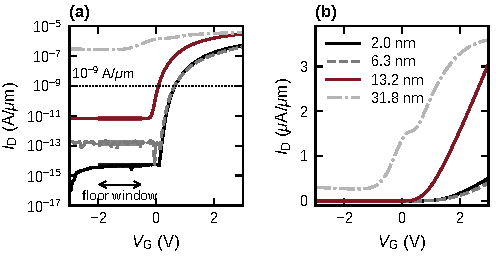
\includegraphics[width=\linewidth]{02_transfer}
      \src{(a) Log scale, line styles as in (b); thick segments: off-state floor (median, $-2 \le \Vg \le -0.5$\,V);
        dotted: $10^{-9}$\,\twoAum. (b) Linear scale. \twoData.}
    \end{column}
    \begin{column}{0.39\textwidth}
      \begin{itemize}\footnotesize
        \item $\Vg$: $-3$ to $+3$\,V, 50\,mV steps, $\Vd = 0.7$\,V; drain current only \lab{measured}\twoC{C001}
        \item 2.0 and 6.3\,nm nearly coincide; 13.2\,nm is shifted to lower $\Vg$, with about six times the
          2.0\,nm on-current \lab{observed}\twoC{C026}
        \item Floors are flat in $\Vg$ and rise steeply with thickness; their origin is open without a gate
          current \lab{observed}
        \item 31.8\,nm never switches off: $\Id(-3\,\mathrm{V}) = 3.0\times10^{-7}$\,\twoAum, on/off about 12
          \lab{derived}\twoC{C029}; outside the published 2--13\,nm series\sref[p.~2]{Januar2026}
      \end{itemize}
    \end{column}
  \end{columns}
  \takeaway{Every trend rests on one sweep of one device per film, with no gate current.}
\end{frame}

% ---------------------------------------------------------------------------------------------------------------------
\begin{frame}[t]{Registered extraction protocol; one disclosed amendment}
  \twoTop
  {\footnotesize
  \renewcommand{\arraystretch}{1.12}
  \begin{tabularx}{\linewidth}{@{}l>{\raggedright\arraybackslash}X@{}}
    \toprule
    Threshold $\Vthcc$ & $\Vg$ at $\Id = 10^{-9}$\,\twoAum{} (290\,nA in total), log-linear interpolation \\
    Off-state floor & median of $\Id$ over $-2 \le \Vg \le -0.5$\,V \\
    Swing (SS) & one decade of current. Registered primary window S1: $[5\times10^{-11}, 5\times10^{-10}]$\,\twoAum;
      secondary window A1, shown here: $[2.15\times10^{-5}, 2.15\times10^{-4}]\,I_\mathrm{on}$,
      $I_\mathrm{on} = \Id(+3\,\mathrm{V})$ \\
    Mobility & $\mu_\mathrm{FE} = L\,g_m/(W C_\mathrm{ox} \Vd)$, $g_m = \partial\Id/\partial\Vg$ (central differences),
      same code for data and simulation; a carrier mobility only if $\Vg - \Vth \ge \Vd$ and $\mu$ is constant \\
    Gate capacitance & $C_\mathrm{ox} = 8.955\times10^{-7}$\,F\,cm$^{-2}$ (EOT 3.86\,nm): 15\,nm \HfO{}
      ($\varepsilon_r$ 19.57) in series with 2\,nm \AlO{} ($\varepsilon_r$ 9.0, assumed) \lab{derived} \\
    \bottomrule
  \end{tabularx}\par}
  \vspace{2mm}
  % timeline: nodes anchored at the baseline of their first line; each dot sits on that first line
  \begin{tikzpicture}[x=1mm,y=1mm,font=\scriptsize,
      tl/.style={anchor=base west,text width=134mm,align=left,inner sep=0pt}]
    \draw[line width=0.5pt] (1,0.75) -- (1,-12.45);
    \fill[ntumaroon] (1,0.75) circle (0.9);
    \fill (1,-4.45) circle (0.7);
    \fill (1,-12.45) circle (0.7);
    \node[tl] at (3.6,0) {6 Oct 2026, decision D-05: protocol committed
      (\texttt{7a61687}), before any data-versus-simulation number of this analysis.};
    \node[tl] at (3.6,-5.2) {After the first results, including the S1
      data--simulation comparison: amendment A1 (\texttt{7ce7116}), as the films' current scales differ.
      Written after its measured values (disclosed), before any simulated value under it.};
    \node[tl] at (3.6,-13.2) {Later (monograph): independent re-implementation
      reproduces thresholds, floors, end-point currents within rounding.};
  \end{tikzpicture}
  \takeaway{Definitions preceded the data--simulation comparison, and A1 preceded any simulated value under it.
    The simulations are calibrated to $\Vthcc$ and $I_\mathrm{on}$: agreement there is not a test.}
\end{frame}

% ---------------------------------------------------------------------------------------------------------------------
\begin{frame}[t]{Threshold is flat to 6.3\,nm, then drops by 0.56\,V}
  \twoTop
  {\centering\footnotesize
  \renewcommand{\arraystretch}{1.0}
  \begin{tabular}{@{}lccccl@{}}
    \toprule
    & 2.0\,nm & 6.3\,nm & 13.2\,nm & 31.8\,nm & \\
    \midrule
    $\Vthcc$ at $10^{-9}$\,\twoAum{} (V) & 0.662 & 0.644 & 0.083 & none & \lab{derived} \\
    Off-state floor (\twoAum) & \num{4.61e-15} & \num{1.53e-13} & \num{6.60e-12} & -- & \lab{derived} \\
    $\Id(+3\,\mathrm{V})$ (\twoAum) & \num{5.09e-7} & \num{4.03e-7} & \num{3.07e-6} & \num{3.59e-6} & \lab{derived} \\
    $\Id(-3\,\mathrm{V})$ (\twoAum) & \num{1.9e-16} & \num{1.9e-13} & \num{6.8e-12} & \num{3.0e-7} & \lab{derived} \\
    $\Id(+3\,\mathrm{V})/\Id(-3\,\mathrm{V})$ & \num{2.7e9}\,$^{\dagger}$ & \num{2.2e6} & \num{4.5e5} & 12
      & \lab{derived} \\
    \bottomrule
  \end{tabular}\par}
  \src{$^{\dagger}$ The 2.0\,nm sweep starts below its floor: not a channel on/off ratio.
    \twoDataShort\sref{Januar2026}; ledger C002, C003, C029; recomputed independently (FACT-101--104).}
  \vspace{-1mm}
  \begin{itemize}\footnotesize
    \item Non-uniform: 2.0\,$\to$\,6.3\,nm changes $\Vthcc$ by $-0.018$\,V and $\Id(+3\,\mathrm{V})$ by $\times0.79$;
      6.3\,$\to$\,13.2\,nm by $-0.561$\,V and $\times7.6$ \lab{observed}\twoC{C026}
    \item The 13.2\,nm floor is 1432 times the 2.0\,nm floor and flat in $\Vg$ within 3\,\%: gate leakage unlikely
      \lab{inferred}\twoC{C005}, but no gate current was recorded
    \item The 2.0\,nm floor, 1.3\,pA in total, is at a measurement-setup level \lab{inferred}\twoC{C003}; no
      instrument floor recorded
  \end{itemize}
  \takeaway{Small change to 6.3\,nm, large to 13.2\,nm: one device per film cannot fix a thickness law.}
\end{frame}

% ---------------------------------------------------------------------------------------------------------------------
\begin{frame}[t]{The published 60--70\,mV/dec appears only next to the floor}
  \twoTop
  \begin{columns}[T,onlytextwidth]
    \begin{column}{0.43\textwidth}
      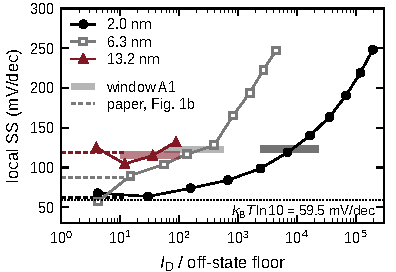
\includegraphics[width=\linewidth]{02_local_ss}
      \src{Local SS $= d\Vg/d\log_{10}\Id$ (central differences), rising branch up to $10^{-9}$\,\twoAum. Bars: window
        A1 and its value. Dashed: paper Fig.~1b value at 1--12 times the floor, where near-floor estimators
        reproduce it; the paper's range is not known. The first 6.3\,nm point lies below $\kT\ln10$, which no
        channel current can do. \twoDataShort.}
    \end{column}
    \begin{column}{0.54\textwidth}
      {\footnotesize
      \setlength{\tabcolsep}{3.5pt}
      \begin{tabular}{@{}lccc@{}}
        \toprule
        SS (mV/dec) & 2.0\,nm & 6.3\,nm & 13.2\,nm \\
        \midrule
        Paper, Fig.~1b & 61.8 & 87.4 & 119.3 \\
        Window A1 & \num{123.6(10)} & \num{122.7(93)} & \num{115.3(24)} \\
        \bottomrule
      \end{tabular}\par}
      \src{Paper values digitised. A1 values derived; A1 is the protocol's secondary window. The registered primary
        window S1 deviates from the paper by up to $+168$\,\% (ledger C008, C032).}
      \begin{itemize}\footnotesize
        \item By its own Fig.~1b, the paper's ``60--70\,mV/dec''\sref[p.~3]{Januar2026} holds at 2.0\,nm only;
          A1 gives twice that \lab{unresolved}\twoC{C025}
        \item Of 31 scored estimator variants, 14 match the paper within 15\,\% if started within 1--12 times the
          floor; the best is an outcome selection, not adopted \lab{derived}\twoC{C032}
        \item A floor $F$ gives $\mathrm{SS}_\mathrm{raw} = \mathrm{SS}_\mathrm{ch}(1 + F/I_\mathrm{ch})$,
          $I_\mathrm{ch}$: channel current. Subtracting $F$ steepens SS by construction; some estimators then fall
          below $\kT\ln10 = 59.5$\,mV/dec at 300\,K \lab{derived}
      \end{itemize}
    \end{column}
  \end{columns}
  \takeaway{Near-thermal switching and a low trap density are not established by these curves.}
\end{frame}

% ---------------------------------------------------------------------------------------------------------------------
\begin{frame}[t]{The \twoMusat{} peak reproduces the published mobilities}
  \twoTop
  \begin{columns}[T,onlytextwidth]
    \begin{column}{0.51\textwidth}
      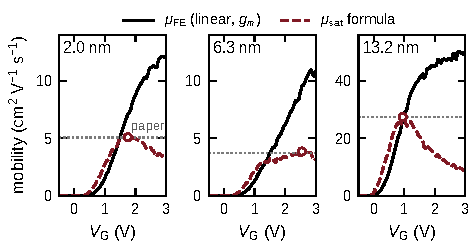
\includegraphics[width=\linewidth]{02_mobility}
      \src{Both formulas on the same curves, $C_\mathrm{ox} = 8.955\times10^{-7}$\,F\,cm$^{-2}$, $W/L = 290/20$,
        $\Vd = 0.7$\,V. Circle: $\mu_\mathrm{sat}$ peak; dotted: paper value. $\mu_\mathrm{sat}$ is one of six
        definitions tested; derivative-estimator spread of its peak 5.04--5.11 / 3.78--3.90 / 25.9--27.5\,\cmVs;
        the $C_\mathrm{ox}$ uncertainty (scales all values) is not included. $\mu_\mathrm{FE}$ peaks at
        $\Vg$ = 3.0 / 2.85 / 2.8\,V. \twoData.}
    \end{column}
    \begin{column}{0.46\textwidth}
      \vspace{-3mm}
      \[ \mu_\mathrm{sat} = \frac{2L}{W C_\mathrm{ox}}\left(\frac{\partial\sqrt{\Id}}{\partial\Vg}\right)^{2} \]\par
      \vspace{-2mm}
      {\footnotesize
      \setlength{\tabcolsep}{4pt}
      \begin{tabular}{@{}lccc@{}}
        \toprule
        cm$^2$\,V$^{-1}$\,s$^{-1}$ & 2.0\,nm & 6.3\,nm & 13.2\,nm \\
        \midrule
        Paper, $\mu_\mathrm{max}$ & 5.1 & 3.73$^{*}$ & 27.4 \\
        $\mu_\mathrm{sat}$ peak & 5.09 & 3.86 & 27.40 \\
        $\mu_\mathrm{FE}$ peak & 12.1 & 10.9 & 50.2 \\
        \bottomrule
      \end{tabular}\par}
      \src{Paper values\sref[pp.~3, 7]{Januar2026}; $^{*}$ digitised from its Fig.~1b. Both lower rows derived.}
      \begin{itemize}\footnotesize
        \item No adjustable factor is needed \lab{derived}\twoC{C030}, so this peak is the leading candidate for
          the paper's definition \lab{inferred}\twoC{C031}
        \item Not an identification: the peaks fix only $C_\mathrm{ox}\,W/L\times$(current unit); $\mu_\mathrm{eff}$
          with power-law threshold and the Y-function also fit, with one common factor (0.68, 0.66)
      \end{itemize}
    \end{column}
  \end{columns}
  \takeaway{A definition difference suffices to reconcile the mobilities; the recipe is unconfirmed.}
\end{frame}

% ---------------------------------------------------------------------------------------------------------------------
\begin{frame}[t]{On linear-regime curves, \twoMusat{} is not a mobility}
  \twoTop
  \begin{columns}[T,onlytextwidth]
    \begin{column}{0.46\textwidth}
      {\footnotesize Linear regime ($V_\mathrm{ov} \ge \Vd$), constant $\mu$, overdrive $V_\mathrm{ov} = \Vg - \Vth$:\par}
      \vspace{-2mm}
      \[ \Id = \mu\,C_\mathrm{ox}\frac{W}{L}\Big(V_\mathrm{ov} - \frac{\Vd}{2}\Big)\Vd \]
      {\footnotesize inserted into the saturation formula:\par}
      \vspace{-2mm}
      \[ \frac{\mu_\mathrm{sat}}{\mu} = \frac{\Vd}{2V_\mathrm{ov} - \Vd} \]
      {\footnotesize Below 1 whenever $V_\mathrm{ov} > \Vd$ and falling as $1/V_\mathrm{ov}$: a low mobility that falls
        with $\Vg$ even when $\mu$ is constant. The saturation formula itself holds only for $V_\mathrm{ov} \le \Vd$.
        \lab{theory}\par}
    \end{column}
    \begin{column}{0.51\textwidth}
      {\footnotesize
      \setlength{\tabcolsep}{4pt}
      \begin{tabular}{@{}lccc@{}}
        \toprule
        At the $\mu_\mathrm{sat}$ peak & 2.0\,nm & 6.3\,nm & 13.2\,nm \\
        \midrule
        $\Vg$ (V) & 1.75 & 2.55 & 0.95 \\
        $V_\mathrm{ov}$ with $\Vthcc$ (V) & 1.09 & 1.91 & 0.87 \\
        $\mu_\mathrm{sat}/\mu_\mathrm{FE}$, constant $\mu$ & 0.47 & 0.22 & 0.68 \\
        $\mu_\mathrm{sat}/\mu_\mathrm{FE}$, observed & 0.72 & 0.41 & 1.02 \\
        \bottomrule
      \end{tabular}\par}
      \src{\twoDataShort\sref{Januar2026}. Ratios derived from the same curves (constant-$\mu$ identity,
        $\Vthcc$); overdrives under all three threshold definitions: ledger C031.}
      \begin{itemize}\footnotesize
        \item With $\Vthcc$ all three peaks lie at $V_\mathrm{ov} > \Vd = 0.7$\,V; with the two other thresholds
          tested, 2.0 and 13.2\,nm can lie inside the range, 6.3\,nm never \lab{derived}
        \item Observed ratios exceed the prediction by 1.5--1.8 \lab{derived}\twoC{M008}, as expected if $\mu$ rises
          with $\Vg$: power-law fits $\mu \propto (\Vg - \Vth)^{\gamma}$ give $\gamma = 0.27\pm0.08$ (13.2\,nm)
          and 1.13 (6.3\,nm) \lab{fitted}\twoC{C011, C012}
      \end{itemize}
    \end{column}
  \end{columns}
  \takeaway{The $\mu_\mathrm{sat}$ peaks are numerical matches, not channel mobilities; nor is $\mu_\mathrm{FE}$
    intrinsic.}
\end{frame}
